CALM captures feature interactions via \emph{conditional feature effects}, a set of univariate shape functions per feature, 
each active in a different region of the input space.

\label{subsec:model-overview}

\textbf{Model formulation.}
Let $\mathbf{X}=(X_1,\ldots,X_d)$ be a random vector with distribution $P_{\mathbf{X}}$ on $\mathcal{X}=\mathcal{X}_1 \times \cdots \times \mathcal{X}_d\subseteq\mathbb{R}^d$, and $\xb=(x_1,\ldots,x_d)$ a point of $\mathcal{X}$.
We use the subscript $-i$ to denote quantities excluding the $i$-th feature (e.g., $\mathbf{X}_{-i}$ defined on $\mathcal{X}_{-i}$). Let also $Y$ be the output random variable, with $Y\in\mathbb{R}$ for regression and $Y\in\{0,1\}$ for binary classification.
CALM is then defined as
\begin{equation}
    \label{eq:CALM}
    g \left ( \mathbb{E}[Y \mid \mathbf{X}=\xb ] \right ) = \beta_0 + \sum_{i=1}^d f_i^{(r_i(\xbi))}(x_i)
\end{equation}
where 
\( \beta_0 \in \mathbb{R} \) is an intercept and
\( g \) is a link function (identity for regression and logit for classification).
For each feature $i$, CALM learns a set of univariate shape functions \( \{ f_i^{(r)} \}_{r=1}^{R_i} \).
At prediction time, a region selection function $r_i: \mathcal{X}_{-i} \to \{1, \ldots, R_i\}$ chooses the specific shape function for $x_i$ based on the context of the other features $\xbi$.
This allows the effect of $x_i$ to vary across regions, effectively modeling feature interactions, while maintaining univariate interpretability within each region.
We denote the prediction of a CALM by $\hat y(\xb)=f_{\texttt{CALM}}(\xb)=g^{-1}\big(\beta_0+\sum_{i=1}^d f_i^{(r_i(\xbi))}(x_i)\big)$.

\textbf{Partition trees.}
Each selection function \( r_i \) partitions $\mathcal{X}_{-i}$, i.e., the input space excluding $x_i$, into regions $\mathcal{P}_i := \{\mathcal{R}_i^{(r)}\}_{r=1}^{R_i}$, independently for each feature $i$.
The goal of these partitions is to minimize interactions between $x_i$ and other features within each region, ensuring the effect of $x_i$ is accurately captured by a single univariate shape function.
Each partition is represented by its own binary decision tree $T_i$ of maximum depth $d_{max}$, built over $\xbi$. 
Internal nodes apply axis-aligned splits, i.e., inequality thresholds \(x_j < \tau\) or $x_j \geq \tau$ for continuous features, and equality tests \( x_j = \tau \) or \(x_j \neq \tau\) for categorical ones. 
Each leaf of the tree defines a region \(\mathcal{R}_i^{(r)}\).
Formally, each region is defined by a conjunction of at most $m_i^{(r)} \leq d_{max}$ rules:
\begin{equation}
\label{eq:region-definition}
\mathcal{R}_i^{(r)} = \left\{ \xbi  \;\middle|\; \textstyle\bigwedge_{k=1}^{m_i^{(r)}} (x_{j_k} \;\text{op}_k\; \tau_k)  \right\}
\end{equation}
where 
\( j_k \in \{1, \dots, d\} \setminus \{i\} \) indexes an interacting feature, 
\( \text{op}_k \in \{<, \geq, =\,, \ne\} \) is a comparison operator,
and
 \( \tau_k \) is a threshold or a category for categorical features.

\textbf{Centering.}
The shape functions are centered at feature level.
In a GAM, each feature has one curve with zero mean over the data, and the intercept $\beta_0$ is the average prediction (on the scale of $g$).
In a CALM, a feature has several curves, so we require them to jointly average to zero:
\begin{equation}
\label{eq:centering-main}
\mathbb{E}\big[f_i^{(r_i(\mathbf{X}_{-i}))}(X_i)\big]
= \sum_{r=1}^{R_i} \mathbb{P}\big(\mathbf{X}_{-i}\in\mathcal{R}_i^{(r)}\big)\,
\mathbb{E}\big[f_i^{(r)}(X_i)\,\big|\,\mathbf{X}_{-i}\in\mathcal{R}_i^{(r)}\big] = 0
\quad \text{for all } i.
\end{equation}
We deliberately avoid centering each curve separately, as this would erase meaningful differences, e.g., the gap between the working-day and day-off curves of the hour in Figure~\ref{fig:concept-image}.

\textbf{High-order interactions.}
As each region conditions on up to $d_{max}$ features, CALM captures interactions of up to $d_{max}+1$ features.
For example, at $d_{max}=2$ the hour of the Bike Sharing data has one curve for working days of the second year ($\mathtt{workingday}=1 \wedge \mathtt{yr}=1$, Figure~\ref{fig:ladder}).
This three-feature interaction is modeled by a univariate curve, whereas a \gamm{} cannot express it at all, and a model with three-way terms would need a 3-D surface.

\textbf{Hyperparameters.}
Increasing $d_{max}$ typically improves accuracy (Section~\ref{sec:complexity}), but at the cost of interpretability.
To balance this trade-off, CALM exposes two hyperparameters: $d_{max}$ (maximum tree depth), which bounds the number of shape functions per feature, $R_i \leq 2^{d_{max}}$, and $K$, which bounds the total number of \emph{conditional interactions} across all trees.
For instance, the three-feature interaction of the Bike Sharing example above counts as two conditional interactions: (hour, working day) and (hour, year).
Two thresholds, $\epsilon$ and $\gamma$, control how readily a split and a tree are accepted (Step~1 of Algorithm~\ref{alg:calm-training}).
In all experiments, we set $d_{max} = 2$, $\epsilon = 0.05$, $\gamma = 0.01$, and leave $K$ unconstrained.

\textbf{Expressivity.}
CALM learns at most $2^{d_{max}}$ curves per feature, yet, since every instance selects one region per feature, these curves combine into up to $\prod_{i} R_i \leq 2^{d\cdot d_{max}}$ distinct additive models.
Fitting these models one by one would split the data into up to $\prod_{i} R_i$ cells, leaving most of them with too few instances. CALM instead shares each curve across all the models whose region it covers, so every curve is still fitted on enough instances: about a $1/R_i$ share of the data for balanced regions.
By contrast, a single tree shared by all features would yield at most $2^{d_{max}}$ additive models.

\subsection{Training algorithm for fitting CALM}
\label{subsec:training}

Given a dataset \( \mathcal{D} = \{(\xb^{(k)}, y^{(k)})\}_{k=1}^N \), we fit a CALM
by minimizing the empirical risk
\( \mathbb{E}_{(\mathbf{X}, Y) \sim \hat{P}_{\mathcal{D}}}\left [ \mathcal{L}(Y, \hat{y}(\mathbf{X})) \right ] \),
where $\mathcal{L}$ is a loss function
and
$\hat{P}_{\mathcal{D}}$ the empirical distribution over $\mathcal{D}$.
This requires estimating
(i) the region selection functions \( r_i \, \forall i \), i.e., a partition tree $T_i$ for each feature, and
(ii) one shape function per region: $\{f_i^{(r)}\}_{r=1}^{R_i}$ and the intercept $\beta_0$.
We solve this problem in two sequential steps summarized in Algorithm~\ref{alg:calm-training}.
\begin{algorithm}[tb]
\caption{Training a CALM model}
\label{alg:calm-training}
\begin{algorithmic}[1]
\renewcommand{\algorithmicensure}{\textbf{Output:}} %
\REQUIRE Training data \( \mathcal{D} = \{(\xb^{(k)}, y^{(k)})\}_{k=1}^N \)
\ENSURE CALM predictor \( f_{\texttt{CALM}}(\xb) \)
\STATE \textbf{Step 1:} Find the regions.
\STATE \quad \textbf{1(a):} Train a reference model \( f_{\texttt{ref}} \) on \( \mathcal{D} \).
\STATE \quad \textbf{1(b):} Propose a tree \( T_i \) for each feature with \( H_i \) at or above the median. \COMMENT{Eq.~\eqref{eq:heterogeneity}, Alg.~\ref{alg:fit-tree}}
\STATE \quad \textbf{1(c):} Select the trees \( \mathcal{S} \) greedily on the surrogate \( R^2 \). \COMMENT{Eq.~\eqref{eq:surrogate-r2}, Alg.~\ref{alg:select-trees}}
\STATE \textbf{Step 2:} Fit the shape functions \( \{ \{f_i^{(r)}\}_{r=1}^{R_i} \}_{i=1}^d \) and \( \beta_0 \). \COMMENT{Alg.~\ref{alg:gb-calm}}
\end{algorithmic}
\end{algorithm}

\textbf{Step 1: Find the regions.}
Step 1 searches for a partition tree $T_i$ per feature such that, within each region, the effect of $x_i$ is well captured by a single univariate shape function, i.e., interactions are locally weak.
It has three substeps:
Step~1(a) trains a reference model,
Step~1(b) \emph{proposes} a tree per feature, and
Step~1(c) \emph{selects} which trees enter the model.

\textit{Step 1(a) Train a reference model.}
We train a high-capacity black-box predictor \( f_{\texttt{ref}} : \mathcal{X} \to \mathbb{R} \) on \( \mathcal{D}\), as a proxy for \( \mathbb{E}[Y | \mathbf{X} ] \).
Any accurate predictor can be used, such as gradient-boosted trees (our default), neural networks, random forests or foundation models like TabPFN \cite{hollmann2022tabpfn}.

\textit{Step 1(b) Propose a tree per feature.}
To find such regions, we use the interaction-related heterogeneity of GADGET~\cite{herbinger2024GADGET}.
Feature effect methods such as PDP or ALE explain a model like $f_{\texttt{ref}}$ through local effects \(h(x_i, \xbi^{(k)})\), the contribution of $x_i$ on instance $\xb^{(k)}$, and average them into a global effect $f_i(x_i)$.
For PDP, our default, the local effect is the centered ICE curve, \(h(x_i, \xbi^{(k)}) = f_{\texttt{ref}}(x_i, \xbi^{(k)}) - \mathbb{E}_{X_i}\left[f_{\texttt{ref}}(X_i, \xbi^{(k)})\right]\).
Heterogeneity is the spread of the local effects around their average: high where $x_i$ interacts with other features, low in near-additive regions.
In a region \(\mathcal{R} \subseteq \mathcal{X}_{-i}\) (e.g., \(\mathcal{R}_i^{(r)}\)), the pointwise heterogeneity of $x_i$ is
\begin{equation}
\begin{aligned}
H_i^{\mathcal{R}}(x_i) &= \mathbb{E}_{\mathbf{X}_{-i}\mid \mathbf{X}_{-i} \in \mathcal{R}}\left[\left ( h(x_i , \mathbf{X}_{-i}) - \mu_i^{\mathcal{R}}(x_i) \right )^2\right]
\end{aligned}
\label{eq:pointwiseh}
\end{equation}
where $\mu_i^{\mathcal{R}}(x_i) = \mathbb{E}_{\mathbf{X}_{-i}\mid \mathbf{X}_{-i} \in \mathcal{R}}\left[h(x_i , \mathbf{X}_{-i})\right]$ and the feature-level heterogeneity is
\begin{equation}
    H^{\mathcal{R}}_i=\sqrt{\mathbb{E}_{X_i|\mathbf{X}_{-i}\in \mathcal{R}}\left[H_i^{\mathcal{R}}(X_i)\right]}
    \label{eq:heterogeneity}
\end{equation}
The square root places $H^{\mathcal{R}}_i$ in the units of the output: it is the typical deviation of a local effect from the average effect of $x_i$ within $\mathcal{R}$.
ALE- and SHAP-DP-based variants are valid alternatives \citep{herbinger2022REPID, herbinger2024GADGET}, and RHALE \citep{gkolemis2023rhale} is preferable under strong feature correlations (Appendix~\ref{subsec:heterogeneity-measures}).
We grow each $T_i$ greedily, in a CART-style fashion, with $H_i^{\mathcal{R}}$ as the criterion.
A tree is proposed only for features whose global heterogeneity $H_i^{\mathcal{X}_{-i}}$ is at or above the median; the others keep a single shape function.
At each node, the split over the conditioning features $x_j \neq x_i$ that most reduces heterogeneity is accepted if the relative reduction exceeds $\epsilon$; otherwise the node becomes a leaf (Appendix~\ref{subsec:partition-tree}).
CART is one choice of partitioner and any other rule learners such as BRL~\citep{letham2015stroke} could replace it.

\textbf{Theoretical justification.}
We show that, under specific assumptions, the error of CALM in approximating $f_{\texttt{ref}}$ is at most $d$ times the sum of the expected squared feature heterogeneities (Proposition~\ref{prop:step2}).
Partitioning to reduce heterogeneity therefore tightens this bound, assuming a perfect fit in Step~2; whether it also lowers the predictive error is an empirical question, addressed in Section~\ref{sec:real-datasets}.

\textit{Step 1(c) Select the trees to keep.}
The trees of Step~1(b) are proposed one feature at a time and are often redundant: an interaction between $x_i$ and $x_j$ raises the heterogeneity of both features, so both trees split on each other, although one suffices.
Keeping every candidate would double-count such interactions and increase the number of curves.
We therefore keep the trees that most improve an additive surrogate of $f_{\texttt{ref}}$.
For a set $\mathcal{S}$ of accepted trees, let $\mathcal{R}_i(\xbi)$ be the region of $T_i$ that $\xbi$ falls in if $i \in \mathcal{S}$, and $\mathcal{X}_{-i}$ otherwise.
The surrogate sums the average local effects $\mu_i^{\mathcal{R}}$ of Eq.~\eqref{eq:pointwiseh} on these regions, and its fidelity to $f_{\texttt{ref}}$ is
\begin{equation}
\label{eq:surrogate-r2}
g_{\mathcal{S}}(\xb) = c_{\mathcal{S}}(\xb) + \sum_{i=1}^d \mu_i^{\mathcal{R}_i(\xbi)}(x_i),
\qquad
R^2(\mathcal{S}) = 1 - \frac{\mathbb{E}\left[\left(f_{\texttt{ref}}(\mathbf{X}) - g_{\mathcal{S}}(\mathbf{X})\right)^2\right]}{\mathrm{Var}\left[f_{\texttt{ref}}(\mathbf{X})\right]},
\end{equation}
where each $\mu_i^{\mathcal{R}}$ is centered over the instances of $\mathcal{R}$, $c_{\mathcal{S}}$ is a piecewise-constant offset over the regions of the trees in $\mathcal{S}$, fitted by least squares, and the expectations are over the training data.
The curves are those already computed in Step~1(b); only $c_{\mathcal{S}}$ is fitted.

Starting from the GAM surrogate ($\mathcal{S} = \emptyset$), each round accepts the candidate with the largest gain in $R^2(\mathcal{S})$ on top of the trees already accepted, provided the gain is at least $\gamma$; selection stops when no candidate clears $\gamma$ or when the next tree would exceed $K$ conditional interactions (Appendix~\ref{subsec:selection}, Algorithm~\ref{alg:select-trees}).
A redundant tree adds almost nothing on top of its partner and is discarded; this is what keeps CALMs small (Section~\ref{sec:real-datasets}), and $K$ only truncates the same sequence.
We stress that $R^2(\mathcal{S})$ measures in-sample fidelity to $f_{\texttt{ref}}$, not predictive accuracy, which is assessed on held-out data in Section~\ref{sec:real-datasets}.
By construction, CALM cannot discover interactions that $f_{\texttt{ref}}$ has not captured; where $f_{\texttt{ref}}$ is near-additive, CALM remains a GAM.

\textbf{Step 2: Fit the shape functions.}
Given the trees, we estimate the region-specific shape functions $\{f_i^{(r)}\}$ and $\beta_0$ by minimizing the empirical risk.
We use a modified gradient boosting in which each iteration updates a single shape function $f_i^{(r)}$, using only the instances whose $\xbi$ falls in $\mathcal{R}_i^{(r)}$ (Algorithm~\ref{alg:gb-calm}).

Although each update is restricted to a single region, the resulting optimization problem is inherently \emph{coupled}.
The regions are defined separately for each feature, so the subsets of samples used to update different shape functions generally overlap.
Consequently, updating one $f_i^{(r)}$ changes the residuals seen by all other shape functions.
Therefore it can be understood as a coordinated optimization of a single additive predictor with region-gated components.

The following proposition characterizes its population target and the convergence of its idealized exact version, which gradient boosting approximates in practice; the proof is in Appendix~\ref{app:step3-theory}.

\begin{proposition}[Optimality and convergence]
\label{prop:step3-main}
Let $m(\xb) = \mathbb{E}[Y \mid \mathbf{X}=\xb]$ denote the true regression function. Assume regression with squared loss, fixed partition trees $\{T_i\}_{i=1}^d$ (as learned by Step~1) and $\mathbb{E}[Y^2]<\infty$.
Let $\mathcal{H}(\{T_i\})$ denote the fixed-tree CALM class (Appendix~\ref{app:step3-theory}), and assume
$\mathcal{H}(\{T_i\})\subset L_2(P_{\mathbf{X}})$ is nonempty, closed, and convex.
Then:
\begin{enumerate}
    \item \emph{Optimality}: 
    Any 
    $s^\star \in \arg\min_{s\in\mathcal{H}(\{T_i\})} \mathbb{E}[(Y-s(\mathbf{X}))^2]$
    is the $L_2(P_{\mathbf{X}})$-best approximation of $m$ within $\mathcal{H}(\{T_i\})$.
    \item \emph{Convergence}: The idealized exact cyclic regional backfitting converges to an empirical risk minimizer over $\mathcal{H}(\{T_i\})$.
\end{enumerate}
\end{proposition}

\subsection{Interpretability of a CALM} \label{subsec:interpretability-properties}
CALMs offer interpretability similar to GAMs, as both require inspecting $d$ univariate plots; one per feature.
CALMs are slightly more complex: unlike GAMs, each plot can contain up to $2^{d_{\text{max}}}$ curves corresponding to a different region of the input space and with interaction-induced discontinuities marked by vertical lines.
However, because regions are interpretable (specified by simple threshold conditions), these region-specific curves provide explanations which are suitable for model auditing and decision support.
For example:
\textit{The effect of the $\mathtt{hour}$ on $\mathtt{rentals}$ follows the working-day curve of Figure~\ref{fig:hero} on a working day and the day-off curve on a day off.}

\textbf{Interpreting a CALM plot.}
In Figure~\ref{fig:hero-calm} each curve gives the contribution of the $\mathtt{hour}$ to $\mathtt{rentals}$ in a specific region;
the orange curve on a working day and the blue curve on a day off.
For example, at 8\,am the contribution is $+246$ (working day) or $-122$ (day off).
The plots also illustrate how altering \( x_i \) to \(x_i \rightarrow x_i + \Delta x \) impacts the prediction.
Vertical dotted lines mark points of a hidden discontinuity which is due to $x_i$ participating as an interaction term for another feature. As shown in Figure~\ref{fig:concept-image}, the effect of the $\mathtt{temperature}$ is conditioned by $\mathtt{hour} \leq 6$ and $\mathtt{hour} \geq 7$ (as is the year's), therefore in Figure~\ref{fig:hero-calm} we observe a vertical line at $6.5$.
If a change in $x_i$ does not cross a vertical line, the change in the output \( (\Delta y) \) equals the curve difference \( (\Delta f_i )\).
Crossing a line signifies a hidden jump, in the range $[\alpha, \beta]$, so 
$ \Delta f_i + \alpha \leq \Delta y \leq \Delta f_i + \beta$.
Arrows provide a fast understanding of the jump:
\(\uparrow\) means $\Delta y > \Delta f_i$,
\(\downarrow\) means $\Delta y < \Delta f_i$,
\(\updownarrow\) means it depends.
The jump at $6.5$ is $[36, 334]$, always \(\uparrow\).
Below, we outline three crucial interpretability properties, along with discussion about their satisfiability by \gam, \gamm, and \method; Figure~\ref{fig:props} answers each on the model of Figure~\ref{fig:hero}. Complete proofs are provided in Appendix~\ref{app:interpretability}.

\begin{figure*}[t]
  \centering
  \begin{subfigure}{0pt}\phantomsubcaption\label{fig:props-p1}\end{subfigure}%
  \begin{subfigure}{0pt}\phantomsubcaption\label{fig:props-p2}\end{subfigure}%
  \begin{subfigure}{0pt}\phantomsubcaption\label{fig:props-p3}\end{subfigure}%
  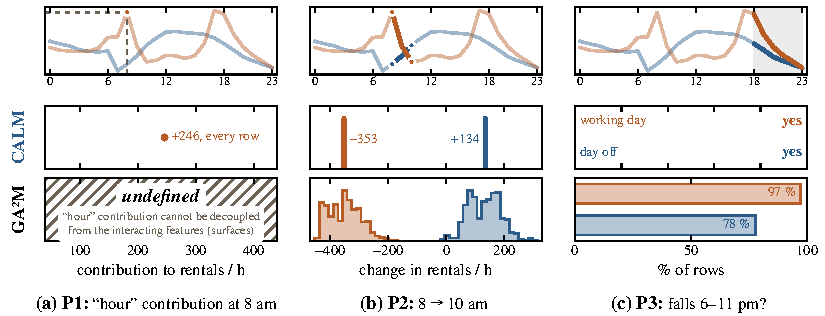
\includegraphics[width=\linewidth]{images/bike/props}
  \caption{The three properties on the model of Figure~\ref{fig:hero}, each asked on every row of the data. Top: CALM's curves, the question marked. CALM's answers are read by eye; the \gamm's are computed, each of the 17{,}379 rows through its eight terms with the hour.
    (\subref{fig:props-p1}) The hour's contribution at 8\,am on a working day: CALM reads $+246$ off the working-day curve, the same on every row; the \gamm's is undefined, since the hour's contribution cannot be decoupled from the interacting features (its seven surfaces).
    (\subref{fig:props-p2}) $\hat{y}(10\,\text{am}) - \hat{y}(8\,\text{am})$: CALM $-353$ on working days and $+134$ on days off, exact on every row since no dotted line is crossed; the \gamm{} spreads from $-430$ to $-257$ and from $+54$ to $+215$ (5th--95th percentile).
    (\subref{fig:props-p3}) Does the prediction fall every hour from 6\,pm to 11\,pm? CALM: yes on working days and days off, since both curves fall and cross no dotted line; the \gamm: on 97\% of working days and 78\% of days off.}
  \label{fig:props}
\end{figure*}


\textbf{P1. Local Feature Contribution:} What is the contribution of each feature to the prediction?\\
\textit{Formally:} Given an input $\xb$, how much does each $x_i$ contribute to $\hat y(\xb)$?\\
The explanation is \emph{local}—it concerns a specific input $\xb$.
In \gam, the contribution is \( f_i(x_i) \).
In \gamm, the contribution is neither explicit nor unique: the pairwise surfaces must be split post hoc, e.g.\ via SHAP or LIME (Figure~\ref{fig:props-p1}).
In \method, the contribution is \( f_i^{(r(\xbi))}(x_i) \).

\textbf{P2. Regional Feature Sensitivity:} How does changing $x_i$ change the prediction? 
\textit{Formally:} Given $x_i$ and $\Delta x>0$, what is $\Delta \hat{y} = \hat y(\xb +  \mathbf{e}_i \Delta x )-\hat y(\xb)$, assuming only $x_i$ is perturbed and $\xbi$ is fixed? 
The explanation is \emph{regional}—it characterizes the effect of $x_i$ on a specific region ($[x_i, x_i + \Delta x]$) \emph{independently} of the values of other features.
In \gam, the change is $\Delta \hat{y} = f_i(x_i+\Delta x)-f_i(x_i)$.
In \gamm, the change depends on every feature that interacts with $x_i$, one surface each (Figure~\ref{fig:props-p2}).
In \method, an exact answer is possible only when the perturbation does not cross a vertical line. 
In this case, the resulting change is a set of values $\Delta y := \{ \Delta f_i^{(r)}\}_{r=1}^{R_i}$, one for each curve in the plot: $\Delta f^{(r)} = f_i^{(r)}(x_i+\Delta x)-f_i^{(r)}(x_i)$. 
If a crossing occurs, an exact answer is not attainable, however, for less precise questions, such as whether the $\Delta x$ change in $x_i$ will have a positive impact on $y$, an answer is still feasible (see \textbf{P3.} below).

\textbf{P3. Global Feature Property:} Is the model globally monotonic increasing with respect to $x_i$?\\ 
\textit{Formally:} For all $\xb$ and $\Delta x>0$, is $\Delta \hat{y} = \hat y(\xb + \mathbf{e}_i \Delta x )-\hat y(\xb) > 0$?\\
The explanation is \textit{global}—it assesses the monotonicity of $x_i$ across the entire input space.
In \gam, monotonicity is easily determined by the shape of $f_i(x_i)$.
In \gamm, every row of every surface $f_{ij}$ must be checked against the curve $f_i$ (Figure~\ref{fig:props-p3}), an inspection infeasible for a human.
In \method, if no vertical lines are present, simply check whether all curves $f_i^{(r)}(x_i)$ for $r=1, \ldots, R_i$ are monotonically increasing. If vertical lines exist, simply verify that all arrows are positive.
